\label{sec:methods}
TODO: methods intro

\subsection{k-Nearest Neighbor Classifier}
The k-Nearest Neighbor (k-NN) classifier is a nonparametric classification technique, which is (generally) used under the assumption that the underlying distribution of the data is unknown. With parametric classification methods, predictions of the unseen data is based on the \emph{fixed parameter models} constructed from the input data. With nonparametric methods, however, the parameter count and nature vary together with the changing data, and the only assumption we can make is the similarity between the input and output data. Various nonparametric methods are available for different machine learning tasks, e.g. classification and regression. \cite{alpaydin:2004:introduction} % p 163

Nonparametric classification algorithms make the decision based the \emph{similarities} between the points to be classified and training data. The definition of the similarity may change between the classification task. One example of similarity measure is the euclidean distance between two points: the closer the points the more similar they are.

The k-NN classifier is a special case of a more general nonparametric classifier. Let us first consider the general nonparametric classification problem. Given a set of N training points  $\mathbf{X} = \{x^{t}\}, t=1...N$, each belonging to a class $\omega_{i}$, we want to assign a point $\mathbf{x} \notin \mathbf{X}$ to one of those classes. In k-NN classifier, the input point is assigned to the class with the most points among the neighbors of the input.

In spite of simplicity, the k-NN classifier is very robust. It is, however, very reliant on the
training data, computationally heavy, and unreliable with higher dimensional data. We believe that the k-NN classifier is suitable for the wine classification task. The size of the training dataset seems large enough to produce meaningful results, and at the same time computationally manageable even with naive implementation. Data pre-processing techniques might be needed to handle the dimensionality and other problems related to the similarity measure. These techniques are discussed in chapters \ref{PCA chapteri}.

% The nonparametric class-conditional density estimate $\hat{p}(\mathbf{x} | \omega_{i})$ for class $\omega_{i}$ is given as

% \begin{equation*}
%   \label{eq:1}
%   \hat{p}(\mathbf{x} | \omega_{i}) = \frac{1}{N_{i}h^{d}} \sum_{t=1}^{N}K(\frac{\mathbf{x} - \mathbf{x}^{t}}{h})\mathbf{r}_{i}^{t}
% \end{equation*}

% where $\mathbf{r}_{i}^{t}$ is 1 when $\mathbf{x^t} \in \omega_{i}$, or 0 otherwise, and $N_{i}$ is the number of data points belonging to $\omega_{i}$. Now, as the maximum likelihood estimate of the prior density $\hat{P}(\omega_{i}) = \frac{N_{i}}{N}$, the discriminant function can be written as

% \begin{equation*}
%   \label{eq:2}
%   g_{i}(\mathbf{x}) = \hat{p}(\mathbf{x}|\omega_{i}) \hat{P}(\omega_{i})
%                     = \frac{1}{Nh^{d}} \sum_{t=1}^{N}K(\frac{\mathbf{x} - \mathbf{x}^{t}}{h})\mathbf{r}_{i}^{t}
% \end{equation*}

% And, since the point is assigned to the class $\omega_{i}$ that maximizes the discriminant, we can ignore the multiplier $1/(Nh^{d})$, and end up with

% \begin{equation}
%   \label{eq:3}
%   g_{i}(\mathbf{x}) = \sum_{t=1}^{N}K(\frac{\mathbf{x} - \mathbf{x}^{t}}{h})\mathbf{r}_{i}^{t}
% \end{equation}

% The intuition behind \eqref{eq:3}, is that each of the training point $\mathbf{x}^t, t = 1...N$, increases the weight of the classified point $\mathbf{x}$, belonging to, and only to, its own class by $K(\frac{\mathbf{x} - \mathbf{x}^{t}}{h})$. The function $K(\cdot)$ is called a kernel function.

% Now, if we limit the estimation to only the k nearest data points, we get

% \begin{equation*}
%   \label{eq:4}
%   \hat{p}(\mathbf{x} | \omega_{i}) = \frac{k_{i}}{N_{i}V^{k}(\mathbf{x})}
% \end{equation*}

% where $k_{i}$ is the number of points belonging to class $\omega_{i}$ and k nearest points of $\mathbf{x}$. $V^{k}(\mathbf{x})$ is the volume of a d-dimensional hypersphere our $\mathbf{x}$. Using bayesian formula, we get

% \begin{equation*}
%   \label{eq:5}
%   \hat{P}(\omega_{i}|\mathbf{x}) = \frac{\hat{p}(\mathbf{x}|\omega_{i})\hat{P}(\omega_{i})}{\hat{p}(\mathbf{x})} = \frac{k_i}{k}
% \end{equation*}


% TODO:
% \begin{itemize}
% \item upper bound for the error
% \item choice of k? cross-validation
% \item zero mean unit variance is required for the euclidean distances!
% \item curse of dimensionality
% \end{itemize}

\subsection{Linear Regression}
In linear regression the relationship between the input variables $\mathbf{X}$ and the predicted variable $\mathbf{y}$ is modeled using a linear combination of basis functions \cite{alpaydin:2004:introduction}. The mathematical expression describing the relationship of the input variables and the predicted variable is given in the equation \ref{eq:666} where input variables are denoted by $\mathbf{X}$, the predicted variable is expressed as a function of input variables $g_{i}(\mathbf{X})$, $\phi$ are the basis functions and $w_{j}$ are the weights for each basis function. The closed form solution for the weights is found using linear algebra. The least squares solution for the weights is given by $\mathbold{w = y\Phi^{\dagger}}$ where $\mathbold{\Phi}$ is a matrix with elements $\phi(x^{t})$ and $\mathbold{\Phi^{\dagger}}$ denotes the pseudo inverse of the matrix \cite{alpaydin:2004:introduction}.

\begin{equation}
    \label{eq:666}
    g_{i}(\mathbf{X}) = \sum^{k}_{j=1}{w_{j}\phi_{ij}(\mathbf{X})}
\end{equation}

When doing regression with single input variable polynomial basis functions are often used. For more than one input variable polynomial regression is rarely used, instead linear basis functions are used. \cite{alpaydin:2004:introduction}

\subsection{Extreme Learning Machine}
Artificial neural networks are a family of machine learning models which consist of multiple locally interconnected, simple computing units called neurons, that together form a network type structure. The neurons can be used to form a non-linear mapping from the input space and dividing a complex problem into simpler subproblems.~\cite{haykin:2009:neural-networks}

The output of the network is adjusted by changing the synaptic weights between the neurons. To obtain the desired behavior of the network, the  weights are learned by a learning algorithm.~\cite{haykin:2009:neural-networks}

Extreme Learning Machines are neural network constructs with two special properties. First, they are single layer feedforward networks, meaning that the neurons connection do not form cycles. Secondly, the weights of the hidden layer are randomly assigned and frozen. These properties have interesting consequenses. The learning algorithm of the weights reduces to a single step, essentially amounting to finding a solution for a linear system. While this results in learning thousands of times faster than traditional backpropagation algorithm~\cite{haykin:2009:neural-networks}, these models can still produce good generalization performance and learn non-trivial, non-linear mappings between the inputs and outputs.~\cite{huang:2006:elm}

Despite the intriguing results shown in the original paper~\cite{huang:2006:elm}, there has been some controversy in the machine learning community, regarding the extreme learning machines and its author.~\cite{reddit:2015:elm-controversy}

\subsection{Support Vector Machines}
Support Vector Machines (SVM) are non-probabilistic supervised learning models that can be used for both classification and regression task. In this paper, we consider only the SVM's used for binary classification.

In the general case, the SVM is used to find the parallel hyperplanes that maximize the marginal between the linearly separable classes, minimizing the classification error. Figure~\ref{fig:support-vector-machine-linear} shows an example of a problem solvable by general SVM.~\cite{theodoridis:2009:pattern-recognition}

\begin{figure}[H]
\centering
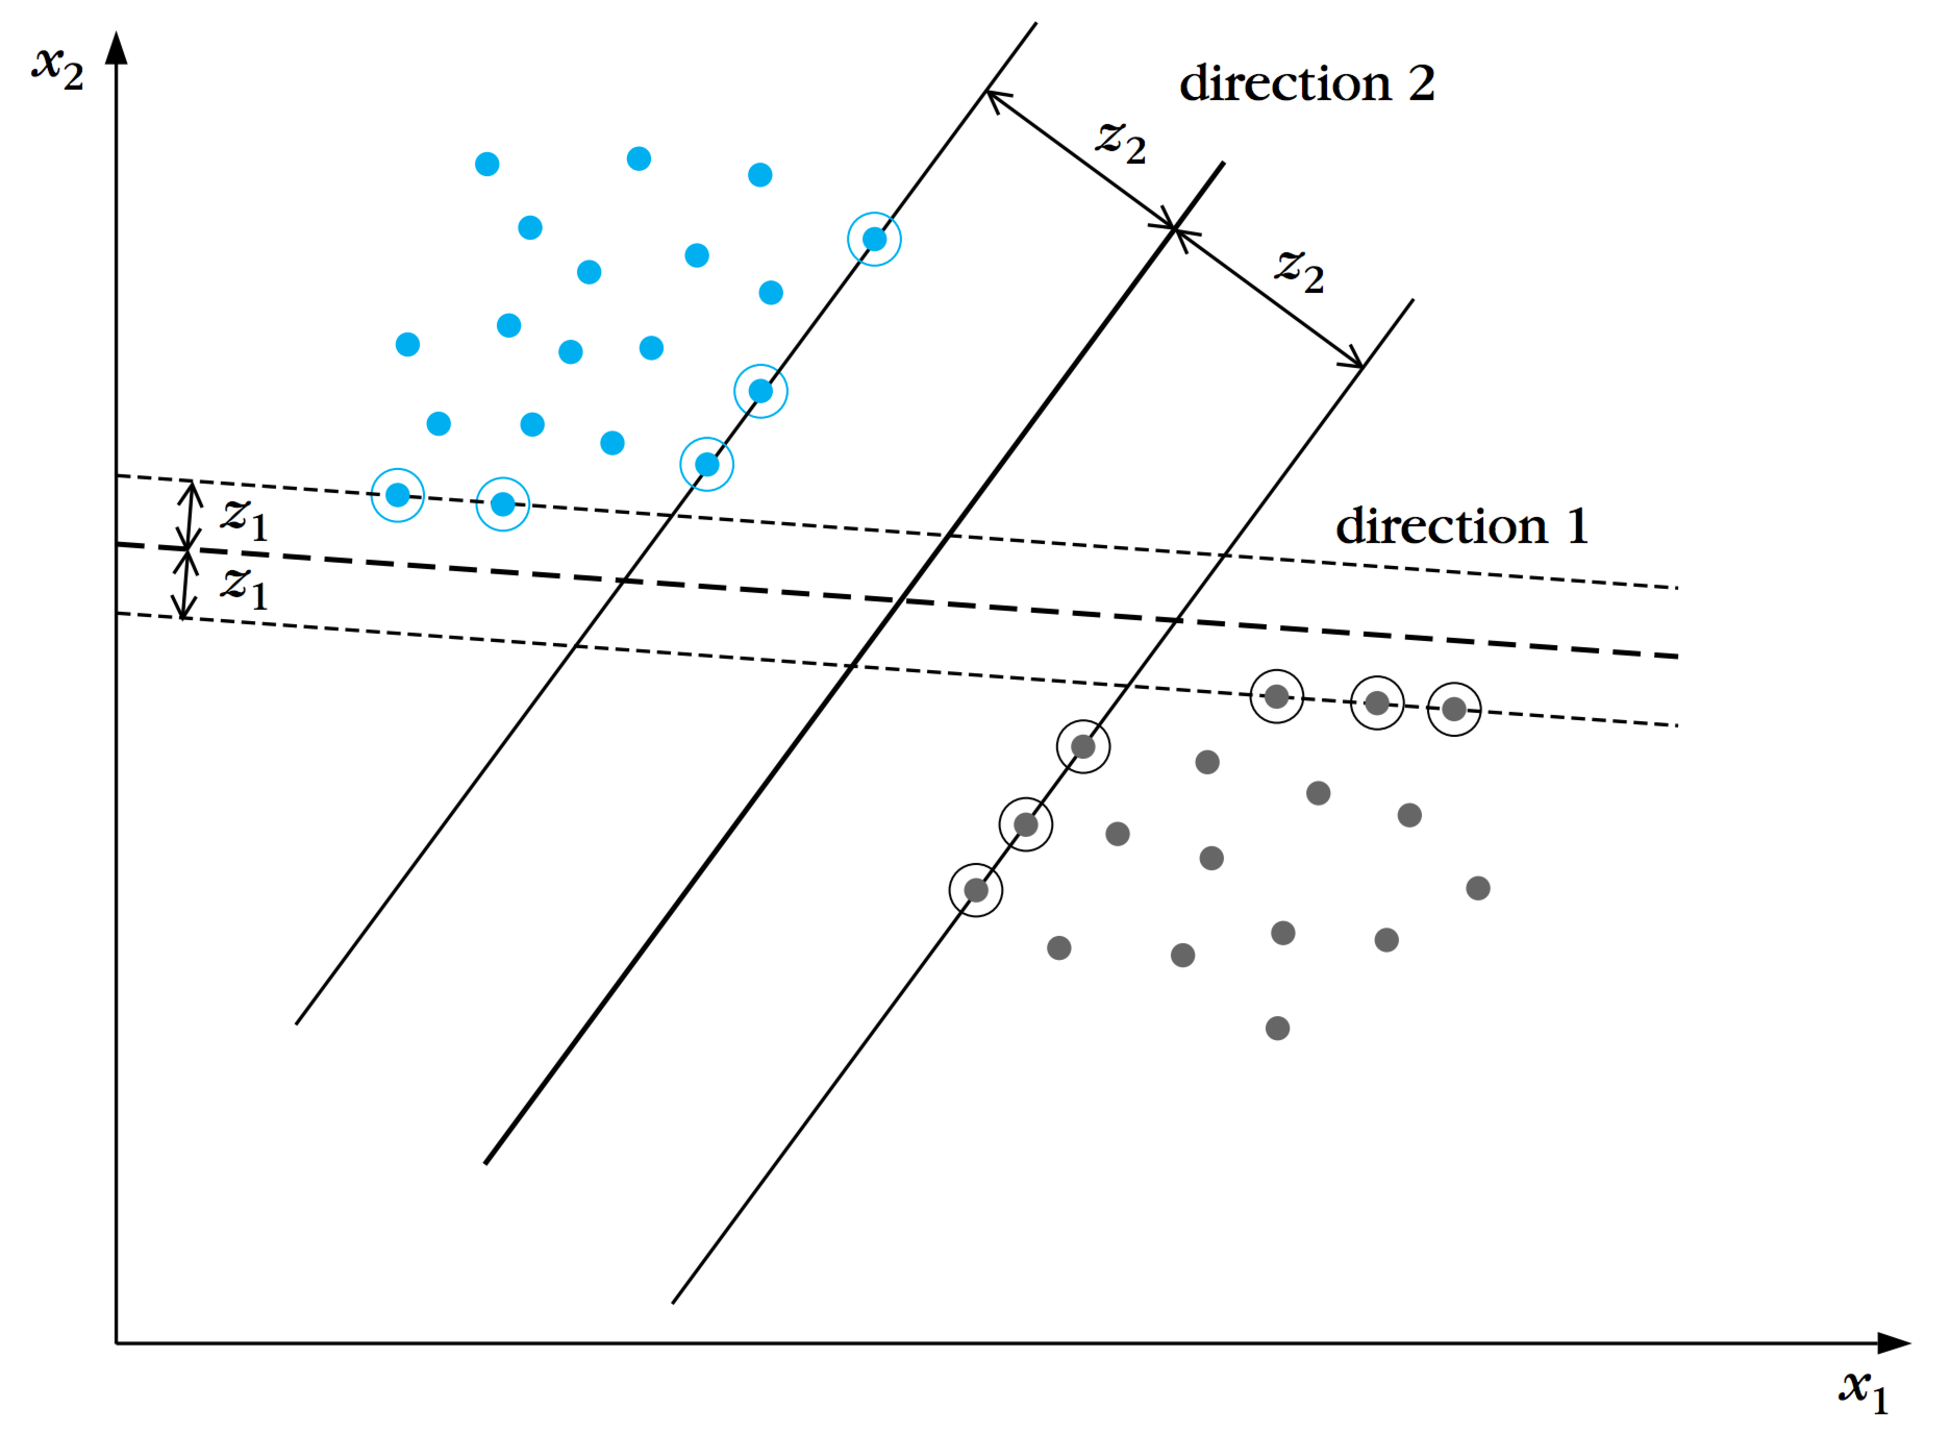
\includegraphics[width=0.48\textwidth]{images/support-vector-machine-linear.pdf}
\caption{An example of a linearly separable binary classification problem with two possible linear classifiers. Support Vector Machine finds the hyperplane that maximises the marginal between the classes.~\cite{theodoridis:2009:pattern-recognition}}
\label{fig:support-vector-machine-linear}
\end{figure}

The general SVM can be extended to solve a non-separable classification problem, by allowing the inputs points to be incorrectly classified with certain cost. Further, a non-linear separation is achieved by non-linearly mapping the input features into a new feature space and using a similar SVM as in the linearly separable case. An example of the non-linear case is presented in the Figure~\ref{fig:support-vector-machine-linear-non-linear}.~\cite{theodoridis:2009:pattern-recognition}

\begin{figure}[H]
\centering
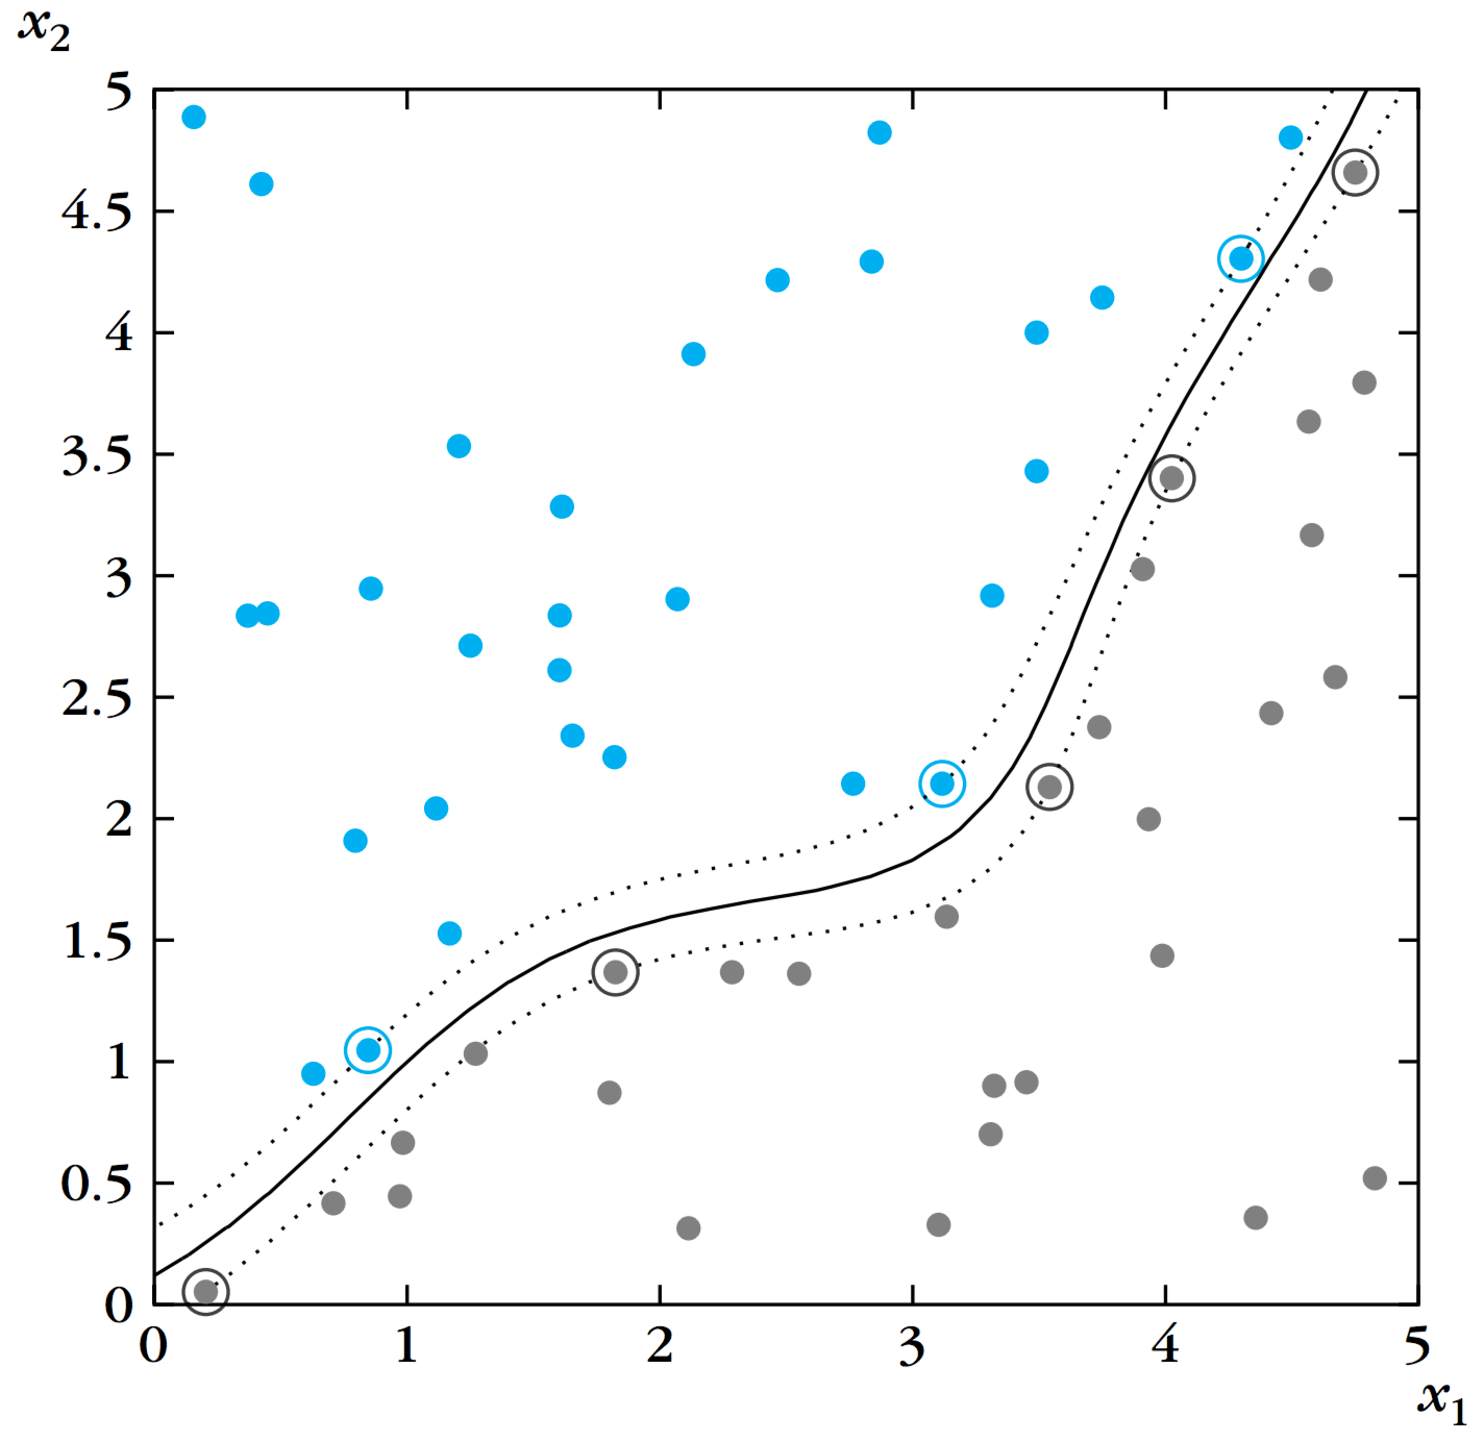
\includegraphics[width=0.48\textwidth]{images/support-vector-machine-non-linear.pdf}
\caption{An example of a classification of non-linear classification done by support vector machine.~\cite{theodoridis:2009:pattern-recognition}}
\label{fig:support-vector-machine-linear-non-linear}
\end{figure}

\subsection{TreeBagger}
One method for creating well performing learners is to combine multiple weaker learners in a way that improves the robustness of the model \cite{alpaydin:2004:introduction}. Combinations of a large number of simpler learners have performed well in machine learning competitions \cite{kaggle:2015:winner}. TreeBagger is a Matlab tool that combines decision trees using bootstrap aggregation \cite{matlab:2015:treebagger}.

The base learning algorithm used by TreeBagger is decision tree. Decision trees are a supervised nonparametric learning method. Decision trees represent the hypothesis by a tree where each leaf node corresponds to an area in the input space. The tree branches are binary decisions. The learning algorithm uses a heuristic method to select the best feature to branch by. The key idea of learning decision trees is to take advantage of the recursive property of trees that a new tree is created by attaching a tree to a leaf of another tree. \cite{alpaydin:2004:introduction}

The empirical error approximates the generalization error the better the larger the dataset is. Because the size of the real training data is limited, the training set is enlarged artificially. One way to artificially enlarge the dataset is to use the histogram of the training data as the ``true'' dataset. Using the histogram for enlarging the dataset is called bootstrap aggregation \cite{breiman:1996:bagging}. TreeBagger uses bagging to create the training datasets for the decision trees.

\subsection{Data Pre-processing}
  - zero mean unit variance
  - feature selection for TreeBagger

\subsection{Model Evaluation}
  - Cross validation

%%% Local Variables:
%%% mode: latex
%%% TeX-master: "report"
%%% End:
